\documentclass[11pt]{article}
\usepackage[letterpaper,margin=1in]{geometry}
\usepackage{mytex}

\usepackage[dvipsnames]{xcolor}
\usepackage[colorlinks=true, citecolor=MidnightBlue, linkcolor=MidnightBlue]{hyperref} % hyperlinks

\usepackage{bookmark}

\usepackage{newtxtext, kotex}
\usepackage[all,cmtip]{xy}
\usepackage{tikz}
\usepackage{tikz-cd}
\usetikzlibrary{calc,positioning}
\usetikzlibrary{arrows.meta,calc,positioning,fit,backgrounds}

\usepackage{pgfplots}
\usepackage{caption}

\usepackage{fancyhdr}
%\fancyhf{} % sets both header and footer to nothing
\renewcommand{\headrulewidth}{0pt}



\usepackage[textwidth=1in,textsize=small,colorinlistoftodos]{todonotes} % todo 노트

\pagestyle{fancy}
\lhead{Myungsin Cho}
\chead{}
\rhead{}
%\rfoot{\date}



%Bibliography line spacing
% ADD THE FOLLOWING COUPLE LINES INTO YOUR PREAMBLE
\let\OLDthebibliography\thebibliography
\renewcommand\thebibliography[1]{
  \OLDthebibliography{#1}
  \setlength{\parskip}{0pt}
  \setlength{\itemsep}{0pt plus 0.3ex}
}

% section 폰트 바꿔주는거
\usepackage{titlesec}
\titleformat{\section}{\normalfont\large\center}{\thesection}{.5em}{}
\titleformat{\subsection}[runin]{\normalfont\bfseries}{\thesubsection}{.5em}{}

\newcommand{\yourname}{Myungsin Cho}

\newcommand\quelle[1]{{%
      \unskip\nobreak\hfil\penalty50
      \hskip2em\hbox{}\nobreak\hfil #1%
      \parfillskip=0pt \finalhyphendemerits=0 \par}}
      

\usepackage{amsmath,amsfonts,amssymb,mathrsfs}
\usepackage{amsthm,thmtools}
\newtheorem{theorem}{Theorem}
\newtheorem{proposition}{Proposition}
\newtheorem{lemma}{Lemma}
\newtheorem{corollary}[theorem]{Corollary}
\newtheorem*{goal}{Goal}
\newtheorem*{conjecture}{Conjecture}

\let\overto\xrightarrow



\author{Myungsin Cho}
\date{}
\begin{document}
\begin{center}\LARGE{Research Statement}\end{center}\vspace{.5em}
%\maketitle
\section*{Introduction}

Duality allows two kinds of information that appear different to determine one another. 
Just as a landscape shapes the trees that grow on it, the trees can also reveal the terrain beneath them. 
My research studies this principle in stable homotopy theory and arithmetic. 
The central goal of my research program is to understand duality in \emph{Real algebraic \(K\)-theory}, with descent serving as one method for recovering global information from local data while retaining symmetry.

My \emph{\(K\)-theoretic duality theorem} for number fields provides the first step in this program. From this starting point, the program moves toward Real algebraic \(K\)-theory in two complementary directions by extending duality to \emph{Grothendieck--Witt theory} and developing \emph{Real trace methods} for computation.

\section{Background}
Topology often turns geometric questions about spaces into algebraic ones. 
Homology studies geometric features of a space, such as connected components, loops, and higher-dimensional holes. 
Cohomology begins from a different point of view. 
It can be viewed as studying function-like algebraic data on a space and how these data fit together globally. 
The \emph{Universal Coefficient Theorem} explains that these two kinds of information are closely related. For example, with coefficients in a field $k$, this relationship takes the particularly simple form
\[
H^n(X;k)\cong \operatorname{Hom}_k(H_n(X;k),k),
\]
Thus, cohomology is the linear dual of homology in this setting. 
This illustrates how duality allows a problem expressed in one kind of information to be understood through another.

Topology also studies spaces and algebraic objects that carry symmetries. 
This raises the complementary question of what information is lost when those symmetries are forgotten. 
Figure~1 shows two different symmetries of a circle. 
After the symmetries are forgotten, the two examples have the same underlying circle. 
Equivariant topology retains this information by studying not only the object itself, but also how its symmetries act and what remains fixed.
\begin{figure}[h]
\centering
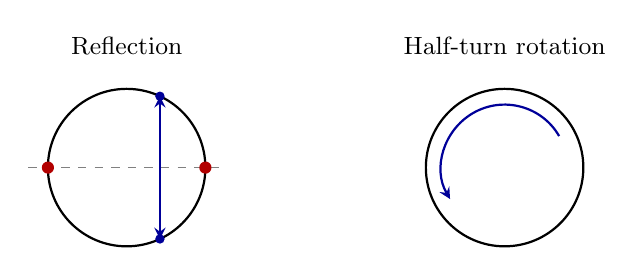
\begin{tikzpicture}[
  >=stealth,
  action/.style={draw=blue!60!black,thick,->},
  fixed/.style={fill=red!70!black},
  orbit/.style={fill=blue!60!black}
]
  % Reflection across the horizontal axis
  \coordinate (L) at (-2.4,0);
  \draw[thick] (L) circle (1);

  % Reflection axis
  \draw[gray,dashed]
    ($(L)+(-1.25,0)$) -- ($(L)+(1.25,0)$);

  % Fixed points
  \fill[fixed] ($(L)+(-1,0)$) circle (2.2pt);
  \fill[fixed] ($(L)+(1,0)$) circle (2.2pt);

  % A pair exchanged by reflection
  \coordinate (Lp) at ($(L)+(65:1)$);
  \coordinate (Lq) at ($(L)+(295:1)$);
  \fill[orbit] (Lp) circle (1.7pt);
  \fill[orbit] (Lq) circle (1.7pt);
  \draw[draw=blue!60!black,thick,<->] (Lp) -- (Lq);

  \node[font=\small] at ($(L)+(0,1.55)$)
    {Reflection};

  % Half-turn rotation
  \coordinate (R) at (2.4,0);
  \draw[thick] (R) circle (1);

  % Semicircular rotation arrow with the same center
  \draw[action]
    ($(R)+(30:0.8)$)
    arc[start angle=30,end angle=210,radius=0.8];

  \node[font=\small] at ($(R)+(0,1.55)$)
    {Half-turn rotation};
\end{tikzpicture}

\captionsetup{font=footnotesize,skip=0.3em}
\caption{Reflection fixes two red points, while rotation by half a turn fixes none.}
\label{fig:circle-actions}
\end{figure}

Questions about duality and symmetry can also be asked for richer topological invariants. 
One such invariant is $K$-theory. 
Topological $K$-theory studies vector bundles over spaces, while algebraic $K$-theory studies their algebraic counterparts, such as projective modules over rings. 
When these objects carry symmetries, $K$-theory can be refined to retain them. 
Atiyah introduced Real $K$-theory to study complex vector bundles together with symmetry modeled on complex conjugation. 
Real algebraic $K$-theory brings this perspective to rings with involution. 
It therefore provides a setting in which duality in algebraic $K$-theory can be studied while retaining symmetry.


\section{Arithmetic Duality and Real Algebraic K-theory}

Real algebraic $K$-theory can be approached through two complementary perspectives. 
Forgetting its $C_2$-symmetry recovers ordinary algebraic $K$-theory, while taking fixed points recovers Grothendieck--Witt theory. 
A duality retaining the full Real structure should therefore appear in both. 
My dissertation establishes the nonequivariant side, and my current work develops the fixed-point side, with the long-term goal of unifying them in a single duality that retains the full $C_2$-equivariant structure.

\subsection{K-theoretic Tate--Poitou duality.}
My dissertation asks whether a classical arithmetic duality has a spectrum-level form in algebraic \(K\)-theory.
The starting point is Tate--Poitou duality, a central cohomological duality for number fields traditionally expressed through étale cohomology.

Although algebraic \(K\)-theory is notoriously difficult to compute, its \(K(1)\)-localization provides a more tractable approximation that retains the arithmetic information relevant here.
Through the Quillen--Lichtenbaum conjecture and the Thomason descent spectral sequence, this approximation is closely connected to étale cohomology \cite{Thomason,MR1697095,MR1803955}.

This makes it natural to expect Tate--Poitou duality to lift to \(K(1)\)-local algebraic \(K\)-theory:
\begin{figure}[h]
\centering
\begin{tikzcd}[column sep=4em, row sep=2em]
%
\textbf{\footnotesize Arithmetic duality:}
\arrow[
    d,
    decorate,
    decoration={
        snake,
        amplitude=0.3mm,
        segment length=2.5mm
    },
    "\text{\scriptsize Descent SS}" right
]
&
|[font=\small]|
{H^\ast_{\mathrm{\acute et}}\!
\bigl(
    \calO_F[\tfrac1p];
    \bZ/p^k(\ast)
\bigr)}
\arrow[d,Rightarrow]
\arrow[
    rr,
    leftrightarrow,
    "\text{\scriptsize Pontryagin dual}"
]
&&
|[font=\small]|
{H^\ast_{c}\!
\bigl(
    \calO_F[\tfrac1p];
    \bZ/p^k(\ast)
\bigr)}
\arrow[d,Rightarrow,dotted]
\\[1ex]
%
\textbf{\footnotesize Homotopical level:}
&
|[font=\small]|
{L_{K(1)}K\bigl(\calO_F[\tfrac1p]\bigr)}
\arrow[
    rr,
    leftrightarrow,
    dotted,
    "\text{\scriptsize spectrum-level duality?}"
]
&&
|[
    fill=PineGreen!4,
    draw=none,
    rounded corners=3pt,
    inner xsep=6pt,
    inner ysep=2pt,
    text=black!75,
    font=\footnotesize,
    align=center
]|
$\begin{gathered}
\text{compactly supported}\\[-1pt]
K\text{-theoretic term}
\end{gathered}$
\end{tikzcd}

\captionsetup{font=footnotesize,skip=0em}
\caption{
Cohomological duality suggests a spectrum-level duality after Thomason descent.
}
\label{fig:duality}
\end{figure}

My dissertation confirms this expectation at the prime \(2\).
\begin{theorem}[\cite{Cho}]\label{mainthm1}
Let \(F\) be a number field. 
The completion cofiber sequence of $K(1)$-local algebraic K-theory admits a canonical \(2\)-adic Anderson self-duality.
The duality acts by reflection across the vertical axis, interchanging the end terms and identifying the middle term with its own dual.
\begin{center}
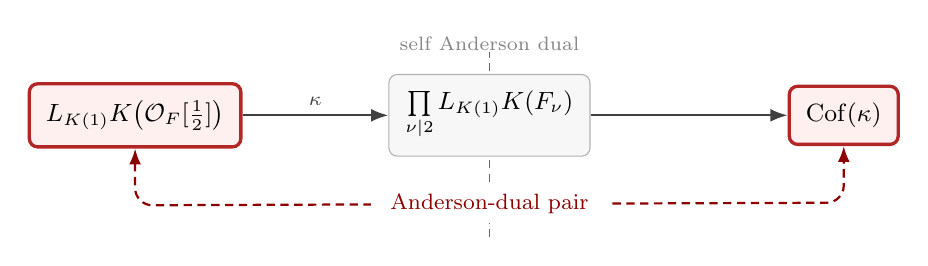
\begin{tikzpicture}[
  >=Latex,
  term/.style={
    draw=black!40,
    fill=black!2,
    rounded corners=3pt,
    inner xsep=6pt,
    inner ysep=6pt,
    align=center,
    font=\small
  },
  main/.style={
    term,
    draw=red!65!black!85!white,
    fill=red!6,
    very thick
  },
  local/.style={
    term,
    draw=black!30,
    fill=black!3
  },
  seq/.style={
    -{Latex[length=2.2mm]},
    thick,
    black!75
  },
  duality/.style={
    {Latex[length=2mm]}-{Latex[length=2mm]},
    thick,
    densely dashed,
    red!55!black
  }
]

\node[main] (global) at (-4.5,0)
  {$L_{K(1)}K\bigl(\mathcal O_F[\tfrac12]\bigr)$};
  
  % Vertical mirror axis
\draw[
  densely dashed,
  black!60
]
  (0,-1.55) -- (0,.8);


\node[local] (local) at (0,0)
  {$\prod\limits_{\nu\mid2}L_{K(1)}K(F_\nu)$};

\node[main] (fiber) at (4.5,0)
  {$\operatorname{Cof}(\kappa)$};

% Completion sequence
\draw[seq]
  (global) --
  node[above,font=\scriptsize] {$\kappa$}
  (local);

\draw[seq]
  (local) -- (fiber);




% Previously known local self-duality
\node[
  above=5pt,
  font=\scriptsize,
  text=black!48
] at (local.north)
  {self Anderson dual};

\draw[duality]
  (global.south)
  -- ($(global.south)+(0,-0.50)$)
  to[out=-90,in=180]
  ($(global.south)+(0.22,-0.72)$)
  --
  node[
    midway,
    fill=white,
    inner xsep=7pt,
    font=\footnotesize,
    text=red!55!black
  ] {Anderson-dual pair}
  ($(fiber.south)+(-0.22,-0.72)$)
  to[out=0,in=-90]
  ($(fiber.south)+(0,-0.50)$)
  -- (fiber.south);
  
 \end{tikzpicture}
\end{center}
\end{theorem}
A homotopy-group-level form of this duality was conjectured by Calegari \cite{MR2905536}.
Blumberg and Mandell later formulated a spectrum-level refinement in terms of \(p\)-adic Anderson duality \(I_{\mathbb Z_p}\), the spectrum-level analogue of Pontryagin duality.
They proved the corresponding local and global duality theorems at every odd prime \cite{MR4121155}.
The theorem above completes the spectrum-level picture at the remaining prime by accounting for the additional cohomological behavior arising from real embeddings.

The case \(F=\bQ\) also yields an application to the algebraic
\(K\)-theory of the sphere spectrum.
Combining the duality theorem with known comparison results gives a
canonical equivalence in nonnegative degrees
\begin{equation*}
\Sigma^{-1}I_{\bZ_2}L_{K(1)}K(\bZ)
\mathrel{\underset{\scriptscriptstyle [0,\infty)}{\simeq}}
\Fib\!\left(
K(\bS)_2^\w
\xrightarrow{\operatorname{trc}_{\bS}}
TC(\bS)_2^\w
\right).
\end{equation*}
Thus, arithmetic information contained in $K(\bZ)$ determines the difference in a fundamental approximation to $K(\bS)$.


\subsection{Grothendieck--Witt theory and  duality.}
Just as algebraic \(K\)-theory is an algebraic analogue of complex vector bundles, Grothendieck--Witt theory plays the role of real vector bundles and records projective modules together with nondegenerate bilinear forms. 
The analogue of forgetting a complex structure on a vector bundle is the hyperbolic map and its fiber defines \(U\)-theory.
\[
U := \Fib\big( K \xrightarrow{\operatorname{hyp}} GW \big)
\]
My current work with Lucy Yang shows that, over \(2\)-adic local fields, this entire sequence exhibits a striking duality symmetry.

\begin{theorem}[\cite{ChoYang}]
Let \(k\) be a 2-adic local field. 
The hyperbolic sequence of $K(1)$-local Grothendieck-Witt theory admits a canonical \(2\)-adic Anderson self-duality.
The duality acts by reflection across the vertical axis, interchanging the end terms and identifying the middle term with its own dual.

\begin{center}
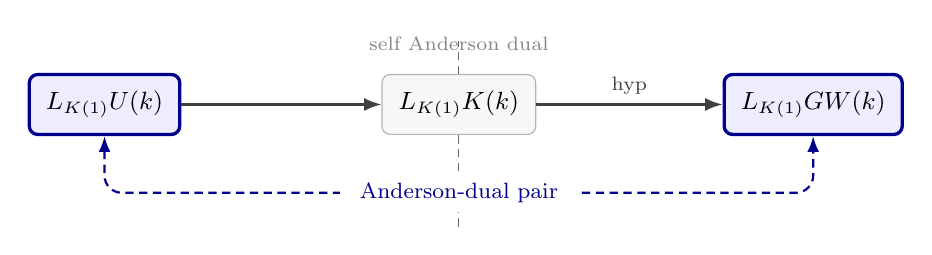
\begin{tikzpicture}[
  >=Latex,
  term/.style={
    draw=black!40,
    fill=black!2,
    rounded corners=3pt,
    inner xsep=6pt,
    inner ysep=6pt,
    align=center,
    font=\small
  },
  main/.style={
    term,
    draw=blue!55!black,
    fill=blue!7,
    very thick
  },
  local/.style={
    term,
    draw=black!30,
    fill=black!3
  },
  seq/.style={
    -{Latex[length=2.2mm]},
    thick,
    black!75
  },
  duality/.style={
    {Latex[length=2mm]}-{Latex[length=2mm]},
    thick,
    densely dashed,
    blue!55!black
  }
]

\node[main] (global) at (-4.5,0)
  {$L_{K(1)}U(k)$};
  
  % Vertical mirror axis
\draw[
  densely dashed,
  black!60
]
  (0,-1.55) -- (0,.8);


\node[local] (local) at (0,0)
  {$L_{K(1)}K(k)$};

\node[main] (fiber) at (4.5,0)
  {$L_{K(1)}GW(k)$};

% Completion sequence
\draw[seq]
  (global) --  (local);

\draw[seq]
  (local) --
node[above,font=\scriptsize] {$\operatorname{hyp}$}
   (fiber);




% Previously known local self-duality
\node[
  above=5pt,
  font=\scriptsize,
  text=black!48
] at (local.north)
  {self Anderson dual};

\draw[duality]
  (global.south)
  -- ($(global.south)+(0,-0.50)$)
  to[out=-90,in=180]
  ($(global.south)+(0.22,-0.72)$)
  --
  node[
    midway,
    fill=white,
    inner xsep=7pt,
    font=\footnotesize,
    text=blue!55!black
  ] {Anderson-dual pair}
  ($(fiber.south)+(-0.22,-0.72)$)
  to[out=0,in=-90]
  ($(fiber.south)+(0,-0.50)$)
  -- (fiber.south);
 
 \end{tikzpicture}
\end{center}
\end{theorem}
 
The local theorem is part of a broader arithmetic picture. In the global setting, the completion sequences for these three theories are expected to assemble into a single self-dual diagram.

\begin{theorem}[Work in progress]
Let \(F\) be a number field.
The completion cofiber sequences for \(U\)-theory, algebraic \(K\)-theory, and GW-theory assemble into a single diagram that is self-dual under \(2\)-adic Anderson duality.
The duality acts by a half-turn, exchanging the \(U\)- and GW-theoretic rows and carrying the \(K\)-theoretic
row to itself.
The middle row recovers \(K\)-theoretic Tate--Poitou duality, while the middle column recovers local GW duality.
\begin{center}
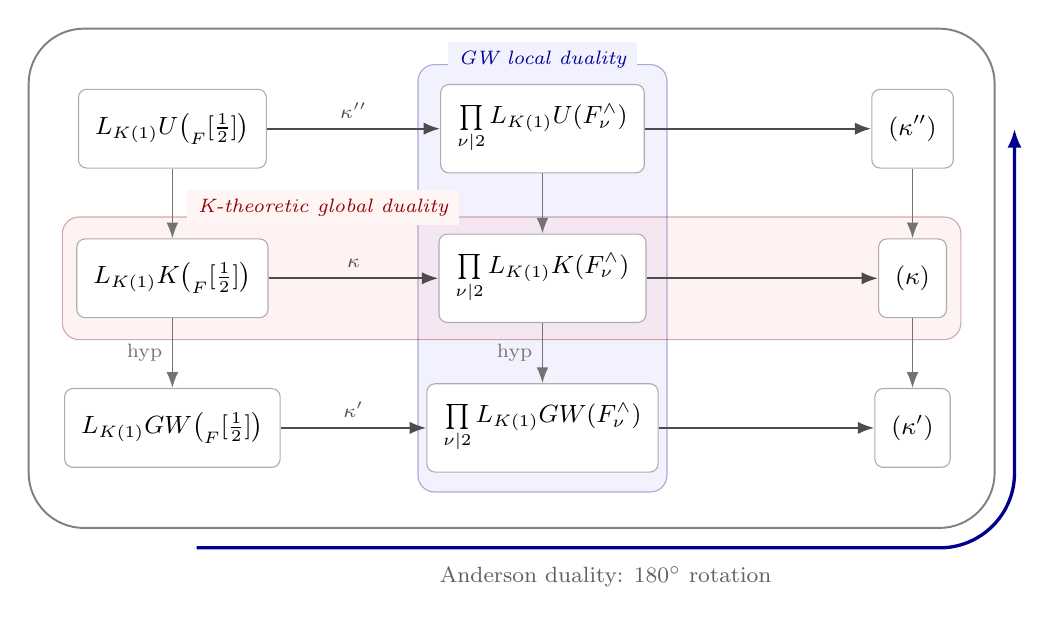
\begin{tikzpicture}[
  >=Latex,
  x=1cm,
  y=1cm,
  term/.style={
    draw=black!32,
    fill=white,
    rounded corners=3pt,
    inner xsep=6pt,
    inner ysep=7pt,
    align=center,
    font=\small,
    minimum height=1.00cm
  },
  seq/.style={-{Latex[length=2.1mm]},thick,black!70},
  vert/.style={-{Latex[length=2mm]},semithick,black!55},
  rotation/.style={{Latex[length=2.4mm]}-,very thick,blue!55!black}
]

% U-row
\node[term] (Ug) at (-4.7,1.9)
  {$L_{K(1)}U\bigl(\calO_F[\tfrac12]\bigr)$};
\node[term] (Ul) at (0,1.9)
  {$\prod\limits_{\nu\mid2}L_{K(1)}U(F_\nu^\wedge)$};
\node[term] (Uc) at (4.7,1.9)
  {$\Cof(\kappa'')$};

% K-row
\node[term] (Kg) at (-4.7,0)
  {$L_{K(1)}K\bigl(\calO_F[\tfrac12]\bigr)$};
\node[term] (Kl) at (0,0)
  {$\prod\limits_{\nu\mid2}L_{K(1)}K(F_\nu^\wedge)$};
\node[term] (Kc) at (4.7,0)
  {$\Cof(\kappa)$};

% GW-row
\node[term] (GWg) at (-4.7,-1.9)
  {$L_{K(1)}GW\bigl(\calO_F[\tfrac12]\bigr)$};
\node[term] (GWl) at (0,-1.9)
  {$\prod\limits_{\nu\mid2}L_{K(1)}GW(F_\nu^\wedge)$};
\node[term] (GWc) at (4.7,-1.9)
  {$\Cof(\kappa')$};

% Horizontal cofiber sequences
\draw[seq] (Ug) -- node[above,font=\scriptsize] {$\kappa''$} (Ul);
\draw[seq] (Ul) -- (Uc);
\draw[seq] (Kg) -- node[above,font=\scriptsize] {$\kappa$} (Kl);
\draw[seq] (Kl) -- (Kc);
\draw[seq] (GWg) -- node[above,font=\scriptsize] {$\kappa'$} (GWl);
\draw[seq] (GWl) -- (GWc);

% Vertical cofiber sequences
\draw[vert] (Ug) -- (Kg);
\draw[vert] (Kg) -- node[left,font=\scriptsize] {$\operatorname{hyp}$} (GWg);
\draw[vert] (Ul) -- (Kl);
\draw[vert] (Kl) -- node[left,font=\scriptsize] {$\operatorname{hyp}$} (GWl);
\draw[vert] (Uc) -- (Kc);
\draw[vert] (Kc) -- (GWc);


% The labels make the two colors self-explanatory.
\node[
  anchor=west,
  font=\scriptsize\itshape,
  text=red!58!black,
  fill=red!4,
  inner xsep=4pt
] at (-4.52,0.9)
  {K-theoretic global duality};

\node[
  anchor=center,
  font=\scriptsize\itshape,
  text=blue!58!black,
  fill=blue!5,
  inner xsep=4pt
] at (0,2.78)
  {GW local duality};


% Backgrounds: the earlier theorem is a horizontal slice of the larger diagram.
\begin{scope}[on background layer]
  \node[
    fit=(Ul)(Kl)(GWl),
    rounded corners=6pt,
    fill=blue!38,
    fill opacity=.13,
    draw=blue!48!black,
    draw opacity=.32,
    inner xsep=3pt,
    inner ysep=7pt
  ] (localslice) {};
  
  \node[
    fit=(Kg)(Kl)(Kc),
    rounded corners=6pt,
    fill=red!38,
    fill opacity=.13,
    draw=red!48!black,
    draw opacity=.32,
    inner xsep=5pt,
    inner ysep=6pt
  ] (kslice) {};

  \node[
    fit=(Ug)(Ul)(Uc)(GWg)(GWl)(GWc)(kslice),
    rounded corners=20pt,
  draw=black!50,
    line width=.7pt,
    inner xsep=12pt,
    inner ysep=20pt
  ] (whole) {};
\end{scope}

\def\dualitygap{0.24}

\draw[
  rotation,
  rounded corners=27pt
]
  ($(whole.east |- Uc.east)+(\dualitygap,0)$)
  -- ($(whole.south east)+(\dualitygap,-\dualitygap)$)
  --
  node[
    midway,
    below=3pt,
    inner xsep=0pt,
    font=\footnotesize,
    text=black!62
  ] {Anderson duality: $180^\circ$ rotation}
  ($(whole.south)+(-4,-\dualitygap)$);
\end{tikzpicture}
\end{center}
\end{theorem}
Thus, the $K$-theoretic Tate--Poitou duality in \autoref{mainthm1} appears as one slice of a larger duality pattern linking $U$-theory, algebraic $K$-theory, and GW-theory.



\subsection{Homological Real trace methods.}
My duality work studies structural relationships in Real algebraic $K$-theory; a complementary challenge is to develop tools for explicit computation.
In joint work with Teena Gerhardt, Liam Keenan, Juan C. Moreno, and J.D. Quigley, I develop \emph{homological Real trace methods} toward this goal \cite{CGKMQ}.
Trace methods replace $K$-theoretic questions by more computable invariants, but in the Real setting the additional $C_2$-symmetry provides new structure that can itself be used in computation.

This extra symmetry already appears in Real topological Hochschild homology.
While ordinary $\operatorname{THH}$ carries the familiar circle action, $\operatorname{THR}$ retains an additional reflection symmetry, as illustrated below.

\begin{figure}[h]
\centering
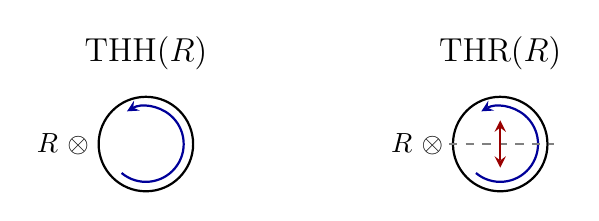
\begin{tikzpicture}[
    >=stealth,
    rotation/.style={draw=blue!60!black,thick,->},
    reflection/.style={draw=red!60!black,thick,<->}
]

% Titles
\node at (-2.25,1.15)
    {\large $\operatorname{THH}(R)$};

\node at (2.25,1.15)
    {\large $\operatorname{THR}(R)$};

% THH center
\coordinate (thh) at (-2.25,0);

% Tensor symbol
\node[anchor=east] at ($(thh)+(-0.6,0)$) {$R\,\,\otimes$};

% THH circle
\draw[thick] (thh) circle (0.6);


% ===== Rotation arrow settings =====
\def\rotstart{-130}   % 시작 각도
\def\rotend{120}    % 끝 각도
\def\rotradius{0.48}

% Rotation arrow
\draw[rotation]
    ([shift=(\rotstart:\rotradius)]thh)
    arc[
        start angle=\rotstart,
        end angle=\rotend,
        radius=\rotradius
    ];


% THR center
\coordinate (thr) at (2.25,0);

% Tensor symbol
\node[anchor=east] at ($(thr)+(-0.6,0)$) {$R\,\,\otimes$};

% THR circle
\draw[thick] (thr) circle (0.6);


% ===== Rotation arrow settings =====
\def\rotstartthr{-130}   % 시작 각도
\def\rotendthr{120}      % 끝 각도
\def\rotradiusthr{0.48}

% Rotation arrow
\draw[rotation]
    ([shift=(\rotstartthr:\rotradiusthr)]thr)
    arc[
        start angle=\rotstartthr,
        end angle=\rotendthr,
        radius=\rotradiusthr
    ];


% ===== Reflection =====

% x-axis reflection axis
\draw[gray, dashed]
    ($(thr)+(-0.65,0)$) -- ($(thr)+(0.68,0)$);

% small vertical reflection arrow
\draw[reflection]
    ($(thr)+(0,-0.30)$) -- ($(thr)+(0,0.30)$);

\end{tikzpicture}
\captionsetup{font=footnotesize}
\caption{
The familiar $\bT$-action on $\operatorname{THH}$ extends in
$\operatorname{THR}$ to an $O(2)\simeq \bT\rtimes C_2$-action.
}
\end{figure}
A key feature of our methods is its compatibility with equivariant multiplicative and power operations, which we use to determine differentials and extract information about the continuous homology of $\operatorname{TCR}^-$.
Technically, this is realized by the following spectral sequence.
\begin{theorem}[\cite{CGKMQ}]
For a $C_2$-equivariant commutative ring spectrum $A$, there is a
natural multiplicative spectral sequence
\[
H_\star\bigl(\operatorname{THR}(A); \ul{\bF}_2\bigr)\langle \bar y\rangle
\Longrightarrow
H^c_\star\bigl(\operatorname{TCR}^-(A); \ul{\bF}_2\bigr),
\]
compatible with equivariant power operations.
For $MU_{\mathbb R}$, $BP_{\mathbb R}$, and several truncated
Brown--Peterson theories, we determine the differentials and the $E_\infty$-page of the resulting spectral sequences.
\end{theorem}

Our construction is a Real refinement of the homological trace methods of Bruner and Rognes \cite{MR2153113}, whose nonequivariant methods became important in the study of Segal conjectures for topological Hochschild homology of $MU$ and $BP$.
Motivated by this work, my long-term goal is to study a Real analogue of the Segal conjecture of $MU_{\mathbb R}$ and $BP_{\mathbb R}$.
This would extend the present calculations toward a broader computational understanding of Real trace invariants and, ultimately, Real algebraic $K$-theory.

The role of genuine equivariant operations in these computations also raises a broader question: which collections of equivariant operations can arise, and how should they be organized?
My work discussed next studies the algebraic and homotopical foundations of this question.


\section{Equivariant algebra: operations and gradings.}
Symmetry changes not only the objects of stable homotopy theory, but also the algebra needed to describe their invariants. 
Genuine equivariant invariants carry richer operations and richer gradings than their nonequivariant counterparts. My work studies these two complementary aspects of equivariant algebra: which equivariant operations can coexist, and how representation-graded information should be organized.

\begin{figure}[h]
\centering
\begin{tikzcd}[column sep=4.5em]
\begin{array}{c}
\textbf{Equivariant operations}
\end{array}
\arrow[d, "\text{\footnotesize encode}"']
&&
\begin{array}{c}
\textbf{Representation gradings}
\end{array}
\arrow[d, "\text{\footnotesize retain}" ]
\\
\begin{array}{c}
\text{transfer systems}\\
\text{$N_\infty$-operads}
\end{array}
&&
\begin{array}{c}
(V,\operatorname{Aut}(V))
\longrightarrow [V]\in RO(C_2)\\[-1mm]
\text{\footnotesize forgetful passage}
\end{array}
\end{tikzcd}
\captionsetup{font=footnotesize}
\caption{
Two complementary aspects of equivariant algebra
}
\label{fig:equivariant-algebra}
\end{figure}
One part of this problem is to understand which equivariant operations can coexist. Transfer systems \cite{MR4244201} provide a combinatorial model for these choices, while $N_\infty$-operads encode the corresponding homotopical structures. In collaboration with David Chan, David Mehrle, Pablo Sanchez Ocal, Ang\'elica Osorno, Ben Szczesny, and Paula Verdugo, we study whether compatibility at the combinatorial level is actually realized homotopically. Our main result establishes one direction in general and a converse in an important case:
\[
\begin{tikzcd}[column sep=8em]
\begin{array}{c}
\text{pairing of}\\[-1mm]
N_\infty\text{-operads}
\end{array}
\arrow[r, Rightarrow, shift left=1.3ex, shorten <=2pt, shorten >=2pt]
&
\begin{array}{c}
\text{compatible pair of}\\[-1mm]
\text{transfer systems}
\end{array}
\arrow[l, dashed, shift left=1ex,
       shorten <=2pt, shorten >=2pt,
       "\text{\footnotesize partially}"]
\end{tikzcd}
\]
\begin{theorem}[\cite{CCM+}]
A pairing of $N_\infty$-operads determines a compatible pair of
transfer systems.  Conversely, if the additive transfer system is
complete, then the compatible pair can be realized by a pairing of
$N_\infty$-operads.
\end{theorem}
We conjecture that the converse holds without this additional assumption and prove several further families of realizable pairs.

Operations are only one part of the story. Equivariant gradings themselves can carry additional structure. 
A basic example comes from equivariant stable homotopy groups, which naturally form Mackey functors.
For a genuine $C_2$-spectrum $X$, its homotopy Mackey functors $\pi_\star X$ are naturally graded by representations of $C_2$. 
While an ordinary $RO(C_2)$-grading records only the class $[V]$ of a representation, Angeltveit and Bohmann introduced the category $\mathcal{RO}(G)$, which refines this grading by retaining morphisms between representation degrees, and in particular the symmetries of a representation $V$ \cite{AngeltveitBohmann}. 
The distinction can be pictured at the level of graded Mackey functors:

\begin{figure}[h]
\centering
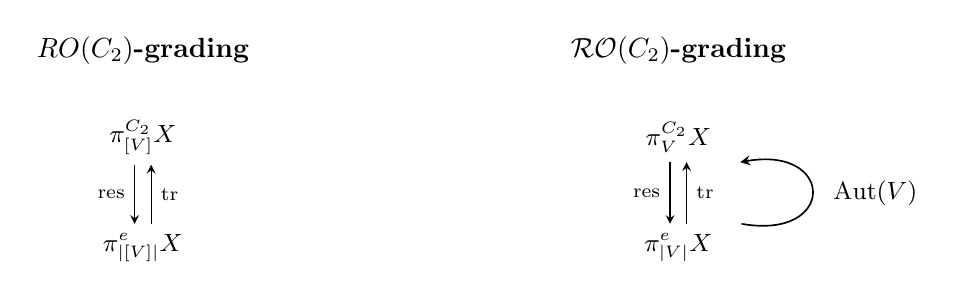
\begin{tikzpicture}[
    every node/.style={font=\small},
    >=stealth
]

% Titles
\node[font=\bfseries] at (-3.4,1.45)
    {$RO(C_2)$-grading};
\node[font=\bfseries] at (3.4,1.45)
    {$\mathcal{RO}(C_2)$-grading};

% Left Lewis diagram
\node (Lt) at (-3.4,0.35)
    {$\pi_{[V]}^{C_2}X$};
\node (Lb) at (-3.4,-1.05)
    {$\pi_{|[V]|}^e X$};

\draw[->]
    ([xshift=-3pt]Lt.south)
    --
    node[left,font=\scriptsize] {$\mathrm{res}$}
    ([xshift=-3pt]Lb.north);

\draw[->]
    ([xshift=3pt]Lb.north)
    --
    node[right,font=\scriptsize] {$\mathrm{tr}$}
    ([xshift=3pt]Lt.south);

% Right Lewis diagram
\node (Rt) at (3.4,0.35)
    {$\pi_V^{C_2} X$};
\node (Rb) at (3.4,-1.05)
    {$\pi_{|V|}^{e}X$};

\draw[->]
    ([xshift=-3pt]Rt.south)
    --
    node[left,font=\scriptsize] {$\mathrm{res}$}
    ([xshift=-3pt]Rb.north);

\draw[->]
    ([xshift=3pt]Rb.north)
    --
    node[right,font=\scriptsize] {$\mathrm{tr}$}
    ([xshift=3pt]Rt.south);

% Action of Aut(V) on the whole graded Mackey functor
\draw[->, semithick]
    ([xshift=7pt]Rb.north east)
    to[out=-10,in=10,looseness=4]
    node[right=4pt,font=\small] {$\operatorname{Aut}(V)$}
    ([xshift=7pt]Rt.south east);

\end{tikzpicture}

\captionsetup{font=footnotesize}
\caption{
$\mathcal{RO}(C_2)$-grading retains the symmetries of the representation
degree $V$.
}
\label{fig:RO-grading}
\end{figure}

In ongoing work with Noah Wisdom, we make this additional structure explicit. We study how $\mathcal{RO}(C_2)$-graded Mackey functors can be described in terms of ordinary $RO(C_2)$-graded data together with the symmetries of the grading, and how this description extends to graded Tambara functors. The goal is to understand how these grading symmetries interact with equivariant operations, providing an algebraic framework for representation-graded coefficient systems arising in genuinely equivariant theories such as Real algebraic $K$-theory.

Together, these projects develop algebraic foundations for working with genuinely equivariant invariants, addressing both the operations they support and the structure carried by their representation gradings. 
These questions also arise naturally in Real algebraic $K$-theory, where genuinely equivariant computational and descent methods require coefficient systems that retain representation-graded information. 
Developing a workable algebraic language for such coefficients is therefore an important step toward understanding how classical descent techniques might extend to the Real setting.





\section{Future research direction}
 
\subsection*{Foundations for Equivariant Algebra}
A key direction of my future work is to develop the basic algebraic framework underlying equivariant stable homotopy theory.
While advanced constructions such as Tambara functors capture much of the structure, many of the elementary notions familiar from commutative algebra remain to be formulated in the equivariant setting.

A natural entry point is the study of commutative $G$-rings, a simpler type of equivariant algebraic object that Tambara functors generalize.
Even in this case, elementary concepts such as algebraic extensions and algebraic closures exhibit subtle equivariant pathologies.
Investigating these questions offers an accessible entry point that also exposes conceptual obstructions in the more general theory of Tambara functors.
Beginning with these manageable cases allows one to develop the algebraic intuition and categorical techniques needed to approach the full equivariant framework.

My goal is to establish such foundational concepts and structures within the equivariant setting.
This foundational program would provide the analogue of commutative algebra for equivariant algebraic geometry, bridging the gap between algebraic and homotopical formulations of equivariant descent.

\subsection*{Undergraduate Research Directions}
Several aspects of my work give rise to problems and projects that are accessible at an undergraduate level yet remain closely connected to broader research questions.
Two areas in particular, combinatorial transfer systems and topological data analysis (TDA), offer tractable problems that both engage students and contribute to the development of my research programs.

One direction of my work focuses on the study of {\it transfer systems} from a combinatorial and educational perspective.  
Because transfer systems are defined directly in terms of subgroup lattices, they are easy to state and visualize, making them particularly suitable for undergraduate research projects.  
At the same time, their enumeration already reveals rich combinatorial structure: for example, the number of transfer systems for cyclic groups coincides with the {\it Catalan numbers} \cite{MR4366744}, and many related patterns remain to be understood.
Exploring these systems provides an accessible way to connect discrete mathematics with deeper questions in equivariant topology.  
Counting and classifying finite posets associated with transfer systems not only offer combinatorial insight but also inform the structural classification of $N_\infty$-operads and Tambara functors, clarifying how discrete data govern admissible algebraic operations.  
In this way, the topic serves both as an entry point for students and as a bridge between combinatorics and the homotopical study of equivariant algebra.

Another area is {\it topological data analysis} (TDA), which applies algebraic topology to study the structure of high-dimensional data sets.
Methods such as {\it persistent homology} can be introduced in a visual and computationally accessible way, yet they lead naturally into deeper questions about stability, functoriality, and the role of cohomology operations.
These connections remain an active area of research, and concrete case studies in TDA provide a natural testing ground for exploring how homotopical invariants can yield new insights into the shape and geometry of data.

In this way, projects in combinatorics and data science serve not only as entry points for undergraduate participation but also as stepping stones toward more advanced problems aligned with my core research agenda.


\bibliography{RS_bib}
\bibliographystyle{alphaurl}

\end{document}